\documentclass[11pt]{article}
\usepackage[margin=1in]{geometry}
\usepackage{amsmath,amssymb,amsthm,mathtools}
\usepackage{microtype}
\usepackage{graphicx}
\usepackage{booktabs}
\usepackage{tikz}
\usetikzlibrary{arrows.meta,positioning,calc}
\usepackage{pgfplots}
\pgfplotsset{compat=1.16}
\usepackage[hidelinks]{hyperref}
\usepackage{xcolor}

\newtheorem{theorem}{Theorem}
\newtheorem{lemma}{Lemma}
\newtheorem{proposition}{Proposition}
\newtheorem{corollary}{Corollary}
\theoremstyle{definition}
\newtheorem{definition}{Definition}
\newtheorem{example}{Example}
\theoremstyle{remark}
\newtheorem{remark}{Remark}

\newcommand{\E}{\mathbb{E}}
\renewcommand{\Pr}{\mathbb{P}}
\newcommand{\logit}{\operatorname{logit}}
\newcommand{\1}{\mathbf{1}}
\newcommand{\Tog}{\mathsf{T}}
\newcommand{\Alo}{\mathsf{A}}

\title{\textbf{Knicks Win Chaos}\\[3pt]
\large Common Knowledge, Coordination, and Equilibrium Routing\\
after a Championship at Madison Square Garden}
\author{Challenge 2 Submission}
\date{}

\begin{document}
\maketitle

\begin{center}
\fbox{\begin{minipage}{0.92\textwidth}
\textbf{Significance.}
When the Knicks win, tens of thousands of fans pour out of Madison Square
Garden into streets that close unpredictably. Getting everyone home is a
problem of \emph{information} and of \emph{coordination}. Following De
Freitas, Thomas, DeScioli, and Pinker \cite{dfp}, we show that what matters
(as Schelling \cite{schelling} anticipated) is not only what each person knows, but what they know that others know.
We prove that (i) official alerts, social media, and public reports fuse
into one closure map by adding log-odds; (ii) selfish routing on a
\emph{shared} map has a unique equilibrium that costs at most $4/3$ of a
perfectly coordinated evacuation; (iii) a coordinated plan (a designated
corridor plus extra trains) works in equilibrium \emph{if and only if} the
plan is approximately common knowledge, which only public broadcasts
create; and (iv) crowd reporting of closures is a volunteer's dilemma whose
outcome zigzags with the level of knowledge, so bigger crowds report less
unless the app breaks the symmetry. A Python prototype implements the model
with a crowd-density map and halves pedestrian exposure to crush-level
densities compared with naive routing.
\end{minipage}}
\end{center}

\begin{abstract}
We model post-game egress as a Bayesian congestion game on a street graph,
with closures as a random state and three information channels (official,
social, crowd) as signals. We prove existence, uniqueness, and a $4/3$
price-of-anarchy bound for equilibrium routing on a public posterior map,
and an exponential bound on the cost of misinformation. We then embed the
stag-hunt and volunteer's-dilemma analyses of \cite{dfp} in this setting:
coordinated egress plans are sustainable exactly on events that are common
$p^*$-belief, and closure reporting follows the private/secondary/tertiary
knowledge zigzag. A density-aware implementation is evaluated on a
synthetic Midtown network.
\end{abstract}

\noindent\textbf{Keywords:} common knowledge $|$ coordination games $|$
Wardrop equilibrium $|$ volunteer's dilemma $|$ crowd routing

%=====================================================================
\section{Introduction}
%=====================================================================

De Freitas et al.\ \cite{dfp} argue that successful coordination requires
\emph{common knowledge}: everyone knows $X$, everyone knows that everyone
knows $X$, and so on. They distinguish \emph{private} knowledge (I know),
\emph{secondary} knowledge (I know you know), \emph{tertiary} knowledge (I
know you know I know), and common knowledge, typically created by a public
broadcast such as a loudspeaker. In a butcher--baker stag hunt, participants
cooperated more as knowledge rose, and most with common knowledge. In a
bystander game, helping zigzagged across knowledge levels as predicted by
the volunteer's dilemma.

A championship night is the same structure at city scale. Fans must choose
routes (a congestion game), the city and transit agencies must decide where
to open corridors and add service (a coordination game), and someone has
to report each closure (a volunteer's dilemma). The challenge asks whether
official alerts, social media, and public reports can map closures and plan
routes home. We answer yes, and identify the knowledge conditions under
which each part works.

%=====================================================================
\section{Model}
%=====================================================================

\paragraph{Network and demand.}
Let $G=(V,E)$ be a directed street graph around the arena, $K$ the set of
origin--destination pairs (arena exits to transit hubs), $d_k>0$ the mass of
travelers for pair $k$, $D=\sum_kd_k$, and $\mathcal P_k$ the simple paths
for pair $k$. A flow $f=(f_P)$ has $f_P\ge0$ and
$\sum_{P\in\mathcal P_k}f_P=d_k$; edge loads are $x_e=\sum_{P\ni e}f_P$.
The feasible set $\mathcal F$ is compact and convex.

\paragraph{Closures and costs.}
The state $\theta\in\{0,1\}^E$ has $\theta_e=1$ if street $e$ is closed,
with independent priors $\Pr(\theta_e=1)=\pi_e\in(0,1)$. Edge costs are
\begin{equation}\label{eq:cost}
c_e(x_e;\theta)=a_ex_e+b_e+M\theta_e,\qquad a_e>0,\ b_e\ge0,
\end{equation}
where $M$ is the time lost reaching a barricade and detouring. Social cost
is $C(f;\theta)=\sum_ex_e\,c_e(x_e;\theta)$.

\paragraph{Information channels.}
For each edge, three signals are conditionally independent given $\theta_e$:
\begin{enumerate}
\item \textbf{Official alert} $O_e\in\{1,\varnothing\}$: issued with
probability $\alpha$ if $\theta_e=1$, never if $\theta_e=0$.
\item \textbf{Social media} $(n_e,k_e)$: $k_e$ of $n_e$ posts claim closure;
each does so with probability $p$ if closed, $q$ if open, $0<q<p<1$.
\item \textbf{Public reports} $(m_e,j_e)$: $j_e$ of $m_e$ reports say
closed; each is correct with probability $r\in(\tfrac12,1)$.
\end{enumerate}
The city publishes the posterior map $\mu_e(s)=\Pr(\theta_e=1\mid s)$ to
everyone, so the map itself is public.

\begin{definition}[Bayesian Wardrop equilibrium]
Given $s$, flow $f^s$ is an equilibrium if every used path for pair $k$
minimizes $\sum_{e\in P}\tilde c_e(x^s_e;s)$ over $\mathcal P_k$, where
$\tilde c_e(x;s)=\E[c_e(x;\theta)\mid s]=a_ex+b_e+M\mu_e(s)$.
\end{definition}

%=====================================================================
\section{Results I: the closure map and selfish routing}
%=====================================================================

\begin{lemma}[Log-odds fusion]\label{lem:fusion}
If $O_e=1$ then $\mu_e=1$. Otherwise
\begin{equation}\label{eq:fusion}
\logit\mu_e=\logit\pi_e+\log(1-\alpha)
+k_e\log\tfrac{p}{q}+(n_e-k_e)\log\tfrac{1-p}{1-q}
+(2j_e-m_e)\log\tfrac{r}{1-r}.
\end{equation}
\end{lemma}

\begin{proof}
Independence across edges makes $\mu_e$ depend only on edge $e$'s signals.
An alert has zero likelihood when $\theta_e=0$, so it forces $\mu_e=1$.
Otherwise Bayes' rule with conditional independence gives the posterior odds
as prior odds times the three likelihood ratios. These are $(1-\alpha)/1$
for no alert; $p^k(1-p)^{n-k}/q^k(1-q)^{n-k}$ for posts; and
$r^j(1-r)^{m-j}/(1-r)^jr^{m-j}=(r/(1-r))^{2j-m}$ for reports (binomial
coefficients cancel). Take logs.
\end{proof}

Each channel casts a weighted vote in log-odds space, and official silence
is mild evidence that a street is open.

\begin{theorem}[Existence and uniqueness \cite{beck}]\label{thm:exist}
For every $s$ an equilibrium exists, and its edge loads $x^s$ are the
unique minimizer over $\mathcal F$ of the Beckmann potential
\[
\Phi_s(x)=\sum_e\int_0^{x_e}\tilde c_e(t;s)\,dt
=\sum_e\Bigl(\tfrac{a_e}{2}x_e^2+(b_e+M\mu_e)x_e\Bigr).
\]
The same holds for any continuous, strictly increasing edge costs,
including the density-based costs of Section~\ref{sec:sim}.
\end{theorem}

\begin{proof}
$\Phi_s$ is continuous on the compact set $\mathcal F$, so a minimizer
exists. Each integral is strictly convex in $x_e$ because its derivative
$\tilde c_e$ is strictly increasing; since $x$ is linear in $f$, the
minimizing load vector is unique. The constraints are linear, so KKT
conditions are necessary and sufficient: with multipliers $\lambda_k$ and
$\nu_P\ge0$, $\sum_{e\in P}\tilde c_e(x_e)=\lambda_k+\nu_P$ and
$\nu_Pf_P=0$. Thus used paths cost exactly $\lambda_k$ and no path costs
less, which is the equilibrium condition. Conversely, an equilibrium
satisfies these KKT conditions with $\lambda_k$ the common used-path cost.
\end{proof}

\begin{lemma}[Bayes consistency]\label{lem:consistency}
For any flow rule $f(s)$ depending only on public signals,
\[
\E[C(f(s);\theta)]=\E\Bigl[\textstyle\sum_ex_e(s)\,\tilde c_e(x_e(s);s)\Bigr].
\]
\end{lemma}

\begin{proof}
Condition on $s$: $x_e(s)$ is $s$-measurable and
$\E[\theta_e\mid s]=\mu_e(s)$. Apply the tower property.
\end{proof}

\begin{theorem}[Price of anarchy on a shared map, cf.\ \cite{rt}]\label{thm:poa}
For any planner flow $f^\star(s)$ using the same signals,
$\E[C(f^s;\theta)]\le\tfrac43\,\E[C(f^\star(s);\theta)]$.
\end{theorem}

\begin{proof}
Fix $s$; write $\tilde c_e(x)=a_ex+\beta_e$ with $\beta_e\ge0$ and
$\tilde C(x)=\sum_ex_e\tilde c_e(x_e)$. Let $x$ be equilibrium loads and $y$
feasible. Optimality of $x$ for convex $\Phi_s$ gives the variational
inequality $\sum_e\tilde c_e(x_e)x_e\le\sum_e\tilde c_e(x_e)y_e$. Since
$(y_e-x_e/2)^2\ge0$,
\[
\tilde c_e(x_e)y_e=a_ex_ey_e+\beta_ey_e\le\tilde c_e(y_e)y_e+\tfrac{a_e}{4}x_e^2
\le\tilde c_e(y_e)y_e+\tfrac14x_e\tilde c_e(x_e).
\]
Summing, $\tilde C(x)\le\tilde C(y)+\tfrac14\tilde C(x)$, so
$\tilde C(x)\le\tfrac43\tilde C(y)$. Take $y=x^\star(s)$, take expectations,
and apply Lemma~\ref{lem:consistency}.
\end{proof}

\begin{theorem}[Cost of an imperfect map]\label{thm:conc}
Let the city publish the MAP map $\hat\theta_e=\1\{\mu_e>\tfrac12\}$ and route
to the equilibrium that treats $\hat\theta$ as true. Suppose each edge gets
at least $m$ (odd) public reports, $\gamma=r-\tfrac12$, and
$\bar C=D\max_{k,P\in\mathcal P_k}\sum_{e\in P}(a_eD+b_e+M)$. Then
\[
\Pr(\hat\theta_e\ne\theta_e)\le(1-\alpha\pi_e)e^{-2m\gamma^2},
\qquad
\E[C(f^{\hat\theta};\theta)]\le\E[C^{\mathrm{FI}}(\theta)]
+\bar C\,e^{-2m\gamma^2}\textstyle\sum_e(1-\alpha\pi_e),
\]
where $C^{\mathrm{FI}}$ is the full-information equilibrium cost.
\end{theorem}

\begin{proof}
Per-edge MAP minimizes per-edge error, so bound the error of the rule
``closed if alert, else majority of reports.'' If $\theta_e=0$ it errs only
if at least half of $m$ reports are wrong, which by Hoeffding has
probability at most $e^{-2m\gamma^2}$. If $\theta_e=1$ it errs only if no
alert ($1-\alpha$) and the majority is wrong, at most
$(1-\alpha)e^{-2m\gamma^2}$. Averaging over the prior gives the first bound.
On $A=\{\hat\theta=\theta\}$ the perceived game equals the true game, so by
uniqueness costs coincide; on $A^c$ costs are at most $\bar C$. Hence
$\E[C]\le\E[C^{\mathrm{FI}}]+\bar C\Pr(A^c)$, and a union bound finishes.
\end{proof}

\begin{corollary}
Any map error has probability at most $\delta$ once
$m\ge\frac{1}{2\gamma^2}\log\frac{|E|}{\delta}$; e.g.\ $|E|=500$,
$r=0.8$, $\delta=0.05$ needs $m\ge52$ reports per segment, fewer with
alerts and posts.
\end{corollary}

%=====================================================================
\section{Results II: coordinated egress needs common knowledge}
%=====================================================================

Selfish routing is a congestion game, but the city's \emph{plan} is a
coordination game. Suppose the MTA and NYPD can open a marshalled corridor
to a station and add trains there, which pays off only if fans actually go
there, while fans gain only if the corridor is actually open. This is the
stag hunt of \cite{dfp} (their Table~1), relabeled in Table~\ref{tab:stag}.

\begin{table}[!htbp]
\centering
\begin{tabular}{lcc}
\toprule
 & Agency: open corridor ($\Tog$) & Agency: default ($\Alo$)\\
\midrule
Fans: use corridor ($\Tog$) & $h,\ h$ & $0,\ 1$\\
Fans: default routes ($\Alo$) & $1,\ 0$ & $1,\ 1$\\
\bottomrule
\end{tabular}
\caption{Egress stag hunt, $h>1$. With the payoffs of \cite{dfp},
$h=1.10$. Both $(\Tog,\Tog)$ and $(\Alo,\Alo)$ are equilibria.}
\label{tab:stag}
\end{table}

\paragraph{Information structure.}
Let $\Omega$ be a finite state space with full-support prior $P$, and
$F\subseteq\Omega$ the event that the corridor plan is feasible (if $F$
fails, $\Tog$ pays $0$). Player $i\in\{1,2\}$ has partition $\Pi_i$. For
$p\in(0,1]$, $i$ \emph{$p$-believes} $E$ at $\omega$ if
$P(E\mid\Pi_i(\omega))\ge p$; write $B_i^p(E)$ for that set. Event $E$ is
\emph{evident $p$-belief} if $E\subseteq B_1^p(E)\cap B_2^p(E)$: whenever it
happens, everyone $p$-believes it. An event is common $p$-belief at $\omega$
iff $\omega$ lies in some evident $p$-belief event \cite{ms}; for $p=1$ this
is common knowledge in the sense of Lewis and Aumann.

Let $p^*=1/h$. Because $\Tog$ pays $h$ only if the other plays $\Tog$ and
$F$ holds, $\Tog$ is a best response at $\omega$ iff
\begin{equation}\label{eq:br}
h\cdot P\bigl(\{\text{other plays }\Tog\}\cap F\mid\Pi_i(\omega)\bigr)\ge1.
\end{equation}

\begin{theorem}[Coordination $\iff$ common $p^*$-belief]\label{thm:ck}
\emph{(a) Necessity.} In any Bayesian equilibrium, let
$T_i\subseteq\Omega$ be where $i$ plays $\Tog$. Then
$E=T_1\cap T_2\cap F$ is evident $p^*$-belief, so successful coordination
only ever happens where $F$ is common $p^*$-belief.

\emph{(b) Sufficiency.} If $E\subseteq F$ is evident $p$-belief with
$p\ge p^*$, there is a Bayesian equilibrium in which both players play
$\Tog$ at every state of $E$.
\end{theorem}

\begin{proof}
(a) $T_i$ is a union of $\Pi_i$-cells. Fix $\omega\in T_i$. By
\eqref{eq:br}, $P(T_j\cap F\mid\Pi_i(\omega))\ge p^*$. Since
$\Pi_i(\omega)\subseteq T_i$, $P(T_i\cap T_j\cap F\mid\Pi_i(\omega))
=P(T_j\cap F\mid\Pi_i(\omega))\ge p^*$, so $T_i\subseteq B_i^{p^*}(E)$.
Since $E\subseteq T_1\cap T_2$, $E\subseteq B_1^{p^*}(E)\cap B_2^{p^*}(E)$.

(b) The game is supermodular: $i$'s gain from $\Tog$ is increasing in the
set where $j$ plays $\Tog$. Let $\sigma^0$ have $i$ play $\Tog$ exactly on
$S_i^0=B_i^p(E)$, which is $\Pi_i$-measurable. Let $\mathrm{BR}$ choose
$\Tog$ when indifferent. For $\omega\in S_i^0$,
$P(S_j^0\cap F\mid\Pi_i(\omega))\ge P(E\mid\Pi_i(\omega))\ge p\ge p^*$,
using $E\subseteq B_j^p(E)=S_j^0$ and $E\subseteq F$. So $\Tog$ is a best
response on $S_i^0$, i.e.\ $S_i^0\subseteq S_i^1:=\mathrm{BR}_i(\sigma^0)$.
By supermodularity, $S^{t}\subseteq S^{t+1}$ implies
$S^{t+1}\subseteq S^{t+2}$, so the $\Tog$-sets increase monotonically. As
$\Omega$ is finite they stabilize at a profile that is its own best
response, an equilibrium with $\Tog$ played on $S_i^\infty\supseteq
B_i^p(E)\supseteq E$.
\end{proof}

With $h=1.10$, $p^*\approx0.91$: the plan must be near-common knowledge.

\begin{corollary}[Which channels can coordinate a plan]\label{cor:channels}
Suppose the plan is announced through channel $c$, a player who receives it
believes the other also received it with probability $\rho_c$, and a player
who did not receive it believes $F$ with probability $\pi_F<p^*$. Then
``play $\Tog$ iff I received the announcement'' is an equilibrium iff
$\rho_c\ge p^*$.
\begin{itemize}
\item Public broadcast (Wireless Emergency Alert to every phone, arena PA,
jumbotron): everyone receives it and sees everyone receive it, so
$\rho=1$; the announcement event is evident $1$-belief, i.e.\ common
knowledge, and coordination succeeds.
\item Social media post: at best secondary knowledge; reach
$\rho_{\text{social}}$ is typically far below $0.91$, so coordination fails.
\item A private report or direct message: private knowledge, $\rho\approx0$.
\end{itemize}
\end{corollary}

\begin{proof}
A non-recipient's payoff from $\Tog$ is at most $h\pi_F<1$, so $\Alo$ is
strictly optimal. A recipient's payoff from $\Tog$ is $h\rho_c$ (the other
plays $\Tog$ exactly when they received it, and $F$ holds when announced),
which is $\ge1$ iff $\rho_c\ge p^*$.
\end{proof}

This reproduces the ordering in Fig.~2 of \cite{dfp}: coordination rises
from private to shared knowledge and peaks with a broadcast. In
Rubinstein's email game \cite{rub}, any \emph{finite} depth of ``I know you
know\dots'' still fails to sustain coordination, which is why the official
plan must be broadcast, not relayed.

%=====================================================================
\section{Results III: who reports the closure?}
%=====================================================================

The map in Theorem~\ref{thm:conc} needs reports, and reporting is the
volunteer's dilemma \cite{dik} that \cite{dfp} use for the bystander
effect. Each of $N$ fans who see a closure may report at cost $\kappa$;
if at least one reports, all gain $B>\kappa$.

\begin{proposition}[Bystander effect under common knowledge]\label{prop:vd}
If the closure and the set of witnesses are common knowledge, the unique
symmetric equilibrium has report probability $p_N=1-(\kappa/B)^{1/(N-1)}$,
and $\Pr_N(\text{no report})=(\kappa/B)^{N/(N-1)}$ is strictly increasing in
$N$, tending to $\kappa/B$.
\end{proposition}

\begin{proof}
Pure symmetric profiles are not equilibria (if nobody reports, deviating
gains $B-\kappa>0$; if everyone reports, deviating saves $\kappa$).
Indifference $B-\kappa=B(1-(1-p)^{N-1})$ gives $(1-p)^{N-1}=\kappa/B$, so
$p_N$ is unique. Then $\log\Pr_N=\frac{N}{N-1}\log\frac{\kappa}{B}$, with
$\log(\kappa/B)<0$ and $\frac{N}{N-1}\downarrow1$, so it increases to
$\log(\kappa/B)$.
\end{proof}

\begin{proposition}[Knowledge-level zigzag]\label{prop:zigzag}
Two fans witness a closure. A fan at level $1$ (private knowledge) believes
the other is unaware; a fan at level $n\ge2$ believes the other is at level
$n-1$, as in the messenger design of \cite{dfp}. An unaware fan never
reports. Then a fan at finite level $n$ reports iff $n$ is odd.
\end{proposition}

\begin{proof}
Induction on $n$. Level 1: the other is unaware and will not report, so
reporting gives $B-\kappa>0$ versus $0$; report. Level $n\ge2$: the other
is at level $n-1$; by induction they report iff $n-1$ is odd. If so, not
reporting yields $B>B-\kappa$; do not report. If $n-1$ is even, the other
does not report, so reporting yields $B-\kappa>0$; report. Hence report iff
$n$ is odd.
\end{proof}

This is the private/secondary/tertiary zigzag found in Fig.~3 of
\cite{dfp}, while the bystander effect of Proposition~\ref{prop:vd}
appears only under common knowledge. Two design rules follow.
\emph{Break the symmetry}: if the app privately pings one witness
(``you're the closest; please confirm''), that fan is at level 1 and
reports with certainty. \emph{Pay for reports}: a reward $\rho\ge\kappa$
makes reporting weakly dominant for all.

\begin{figure}[!htbp]
\centering
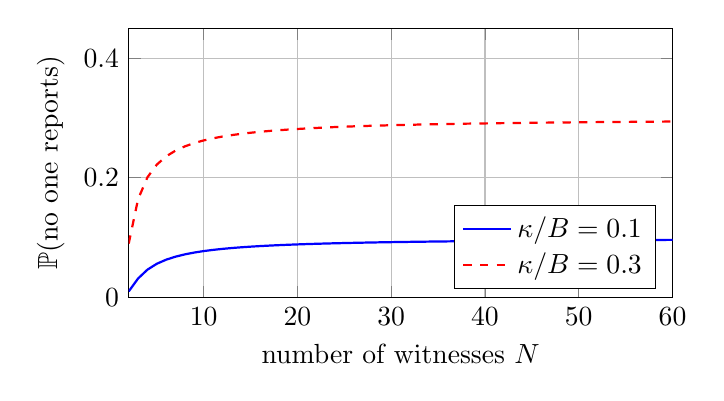
\begin{tikzpicture}
\begin{axis}[width=0.7\textwidth,height=5cm,
  xlabel={number of witnesses $N$},ylabel={$\Pr(\text{no one reports})$},
  xmin=2,xmax=60,ymin=0,ymax=0.45,legend pos=south east,grid=major,
  every axis plot/.append style={thick,samples=59,domain=2:60}]
\addplot[blue]{0.1^(x/(x-1))}; \addlegendentry{$\kappa/B=0.1$}
\addplot[red,dashed]{0.3^(x/(x-1))}; \addlegendentry{$\kappa/B=0.3$}
\end{axis}
\end{tikzpicture}
\caption{Proposition~\ref{prop:vd}: under common knowledge, larger crowds
leave closures unreported more often.}
\end{figure}

%=====================================================================
\section{Results IV: density-aware routing prototype}\label{sec:sim}
%=====================================================================

The accompanying script \texttt{knicks\_router.py} implements the model on
a Midtown grid (5th--10th Ave, W 26th--W 45th St) with exits around the
Garden and five transit destinations.

\paragraph{Density map.} A Gaussian kernel density estimate of (simulated)
phone pings around celebration hot spots gives a crowd density field
$\rho_0(x,y)$ in persons/m$^2$. Routed fans add density
$\Delta\rho_e(f_e)=f_e\,\tau_e/(T\,L_e w)$, where $\tau_e$ is free-walk
time, $T$ the egress window, $L_e$ length, and $w$ walkable width.

\paragraph{Edge cost.} Walking speed follows the Greenshields fundamental
diagram $v(\rho)=v_f(1-\rho/\rho_{\mathrm{jam}})$ (floored at $v_{\min}$),
with $v_f=1.34$\,m/s and $\rho_{\mathrm{jam}}=5.4$\,persons/m$^2$, so
\[
c_e(f_e)=\frac{L_e}{\max\{v_{\min},\,v_f(1-(\rho_{0,e}+\Delta\rho_e(f_e))/\rho_{\mathrm{jam}})\}}
+M\mu_e .
\]
This is continuous and increasing in $f_e$, so Theorem~\ref{thm:exist}
guarantees a unique equilibrium. (The $4/3$ bound of
Theorem~\ref{thm:poa} is specific to affine costs.)

\paragraph{Closure map and assignment.} Signals are simulated per street
and fused by Lemma~\ref{lem:fusion}. Equilibrium is computed by the method
of successive averages, which converges for separable increasing costs
\cite{sheffi}; the final relative gap is $0.003\%$.

\begin{table}[!htbp]
\centering
\begin{tabular}{lrrr}
\toprule
Routing strategy & trip (min) & into barricades & blocks at $>2$ p/m$^2$\\
\midrule
Naive shortest path & 24.8 & 13{,}200 & 40{,}000\\
Closure-aware (fused signals) & 15.7 & 0 & 25{,}980\\
Closure + density-aware equilibrium & 15.4 & 0 & 19{,}975\\
\bottomrule
\end{tabular}
\caption{Synthetic evaluation (20{,}000 fans, seed 7), scored under the
true closures. The fused map detected all 14 directed closed segments with
2 false alarms. Density awareness barely changes trip time but cuts
exposure to crush-risk densities by $23\%$ versus closure-only and $50\%$
versus naive routing.}
\label{tab:sim}
\end{table}

\begin{figure}[!htbp]
\centering
\includegraphics[width=0.78\textwidth]{knicks_routes.png}
\caption{Output of \texttt{knicks\_router.py}: crowd density (heat map),
inferred closures (red), and equilibrium walking flows (blue, width
proportional to fans).}
\end{figure}

%=====================================================================
\section{Discussion}
%=====================================================================

\emph{Could official alerts, social media updates, and public reports help
map street closures and plan alternate routes home?} Yes, with a division
of labor dictated by levels of knowledge:
\begin{enumerate}
\item \textbf{Mapping} uses all three channels, fused by
Lemma~\ref{lem:fusion}; errors vanish exponentially in report volume
(Theorem~\ref{thm:conc}).
\item \textbf{Routing} works on a \emph{shared} map, with a unique
equilibrium within $4/3$ of optimal (Theorems~\ref{thm:exist},
\ref{thm:poa}), and density-aware costs reduce crowd crush risk.
\item \textbf{Coordinated plans} (corridors, extra trains) must be
\emph{broadcast} to create common knowledge (Theorem~\ref{thm:ck},
Corollary~\ref{cor:channels}); social media alone cannot do it.
\item \textbf{Reporting} must be designed around the volunteer's dilemma:
ping individual witnesses or reward reports
(Propositions~\ref{prop:vd}, \ref{prop:zigzag}).
\end{enumerate}

\paragraph{Limitations.} Signals are assumed conditionally independent
(retweets violate this); closures are exogenous, though crowds create
them; the knowledge-level model of Proposition~\ref{prop:zigzag} is the
stylized hierarchy of \cite{dfp}; and the simulation uses synthetic data
and approximate block lengths.

\begin{thebibliography}{9}
\bibitem{dfp} J.~De Freitas, K.~Thomas, P.~DeScioli, S.~Pinker, Common
knowledge, coordination, and strategic mentalizing in human social life.
\emph{Proc. Natl. Acad. Sci. U.S.A.} 116, 13751--13758 (2019).
\bibitem{ms} D.~Monderer, D.~Samet, Approximating common knowledge with
common beliefs. \emph{Games Econ. Behav.} 1, 170--190 (1989).
\bibitem{rub} A.~Rubinstein, The electronic mail game: strategic behavior
under ``almost common knowledge.'' \emph{Am. Econ. Rev.} 79, 385--391 (1989).
\bibitem{dik} A.~Diekmann, Volunteer's dilemma. \emph{J. Conflict
Resolut.} 29, 605--610 (1985).
\bibitem{schelling} T.~C.~Schelling, \emph{The Strategy of Conflict}
(Harvard Univ. Press, 1960).
\bibitem{beck} M.~Beckmann, C.~B.~McGuire, C.~B.~Winsten, \emph{Studies in
the Economics of Transportation} (Yale Univ. Press, 1956).
\bibitem{rt} T.~Roughgarden, \'E.~Tardos, How bad is selfish routing?
\emph{J. ACM} 49, 236--259 (2002).
\bibitem{sheffi} Y.~Sheffi, \emph{Urban Transportation Networks}
(Prentice-Hall, 1985).
\end{thebibliography}

\end{document}
